\appendix 
\onecolumn
%\icmltitle{Supplementary Material \\ Random Feature Expansions for Deep Gaussian Processes}

\section{Additional Experiments}

Using the experimental set-up described in Section 4, Figure~\ref{fig:mnll_vs_time} demonstrates how the competing models perform with regards to the \rmse (or error rate) and \mnll metric when two hidden layers are incorporated into the competing models.
The results follow a similar progression to those reported in Figure~3 of the main paper.
The \dgparc and \dgprbf models both continue to perform well after introducing this additional layer.
However, the results for the regularized \dnn are notably inferior, and the degree of overfitting is also much greater.
To this end, the \mnll obtained for the \mnist dataset is not shown in the plot as it was vastly inferior to the values obtained using the other methods.
\dgpep was also observed to have low scalability in this regard whereby it was not possible to obtain sensible results for the \mnist dataset using this configuration.
 
\input{figures/comparison_3l}

In Section 3.3, we outlined the different strategies for treating $\Omegavect$, namely fixing them or treating them variationally, where we observed that the constructed \dgp model appears to work best when these are treated variationally while fixing the randomness in their computation throughout the learning process (\name{var-fixed}).
In Figures~\ref{fig:optim_error} and~\ref{fig:optim_mnll}, we compare these three approaches on the complete set of datasets reported in the main experiments for one and two hidden layers, respectively.
Once again, we confirm that the performance obtained using the \name{var-fixed} strategy yields more consistent results than the alternatives.
This is especially pertinent to the classification datasets, where the obtained error rate is markedly superior.
However, the variation of the model constructed with the \arccosine kernel and optimized using \name{var-fixed} appears to be susceptible to some overfitting for higher dimensional datasets (\spam and \mnist), which is expected given that we are optimizing several covariance parameters (\ard).
This would motivate trying to be variational about $\Thetavect$ too. 

\input{figures/comparison_models_2l}
\input{figures/comparison_models_3l}

\section{Comparison with \mcmc}

Figure~\ref{fig:compare_MCMC_variational} shows a comparison between the variational approximation and \mcmc for a two-layer \dgp model applied to a regression dataset.
The dataset has been generated by drawing $50$ data points from $\norm(y | h(h(x)), 0.01)$, with $h(x) = 2x \exp(-x^2)$.
We experiment with two different levels of precision in the \dgp approximation by using $10$ and $50$ fixed spectral frequencies, respectively, so as to assess the impact on the number of random features on the results.
%% In order to be consistent with the visualization of the results obtained by the \mcmc sampler, we fixed the $\Omega^{(i)}$ weight matrices, as optimizing them variationally may not preserve the property that $\Phi^{(i)} \left(\Phi^{(i)}\right)^{\top}$ unbiasedly approximates the corresponding covariance $K^{(i)}$.
For \mcmc, covariance parameters are fixed to the values obtained by optimizing the variational lower bound on the marginal likelihood in the case of $50$ spectral frequencies.


\begin{figure}[ht]
%% \vspace{.3in}
\centerline{
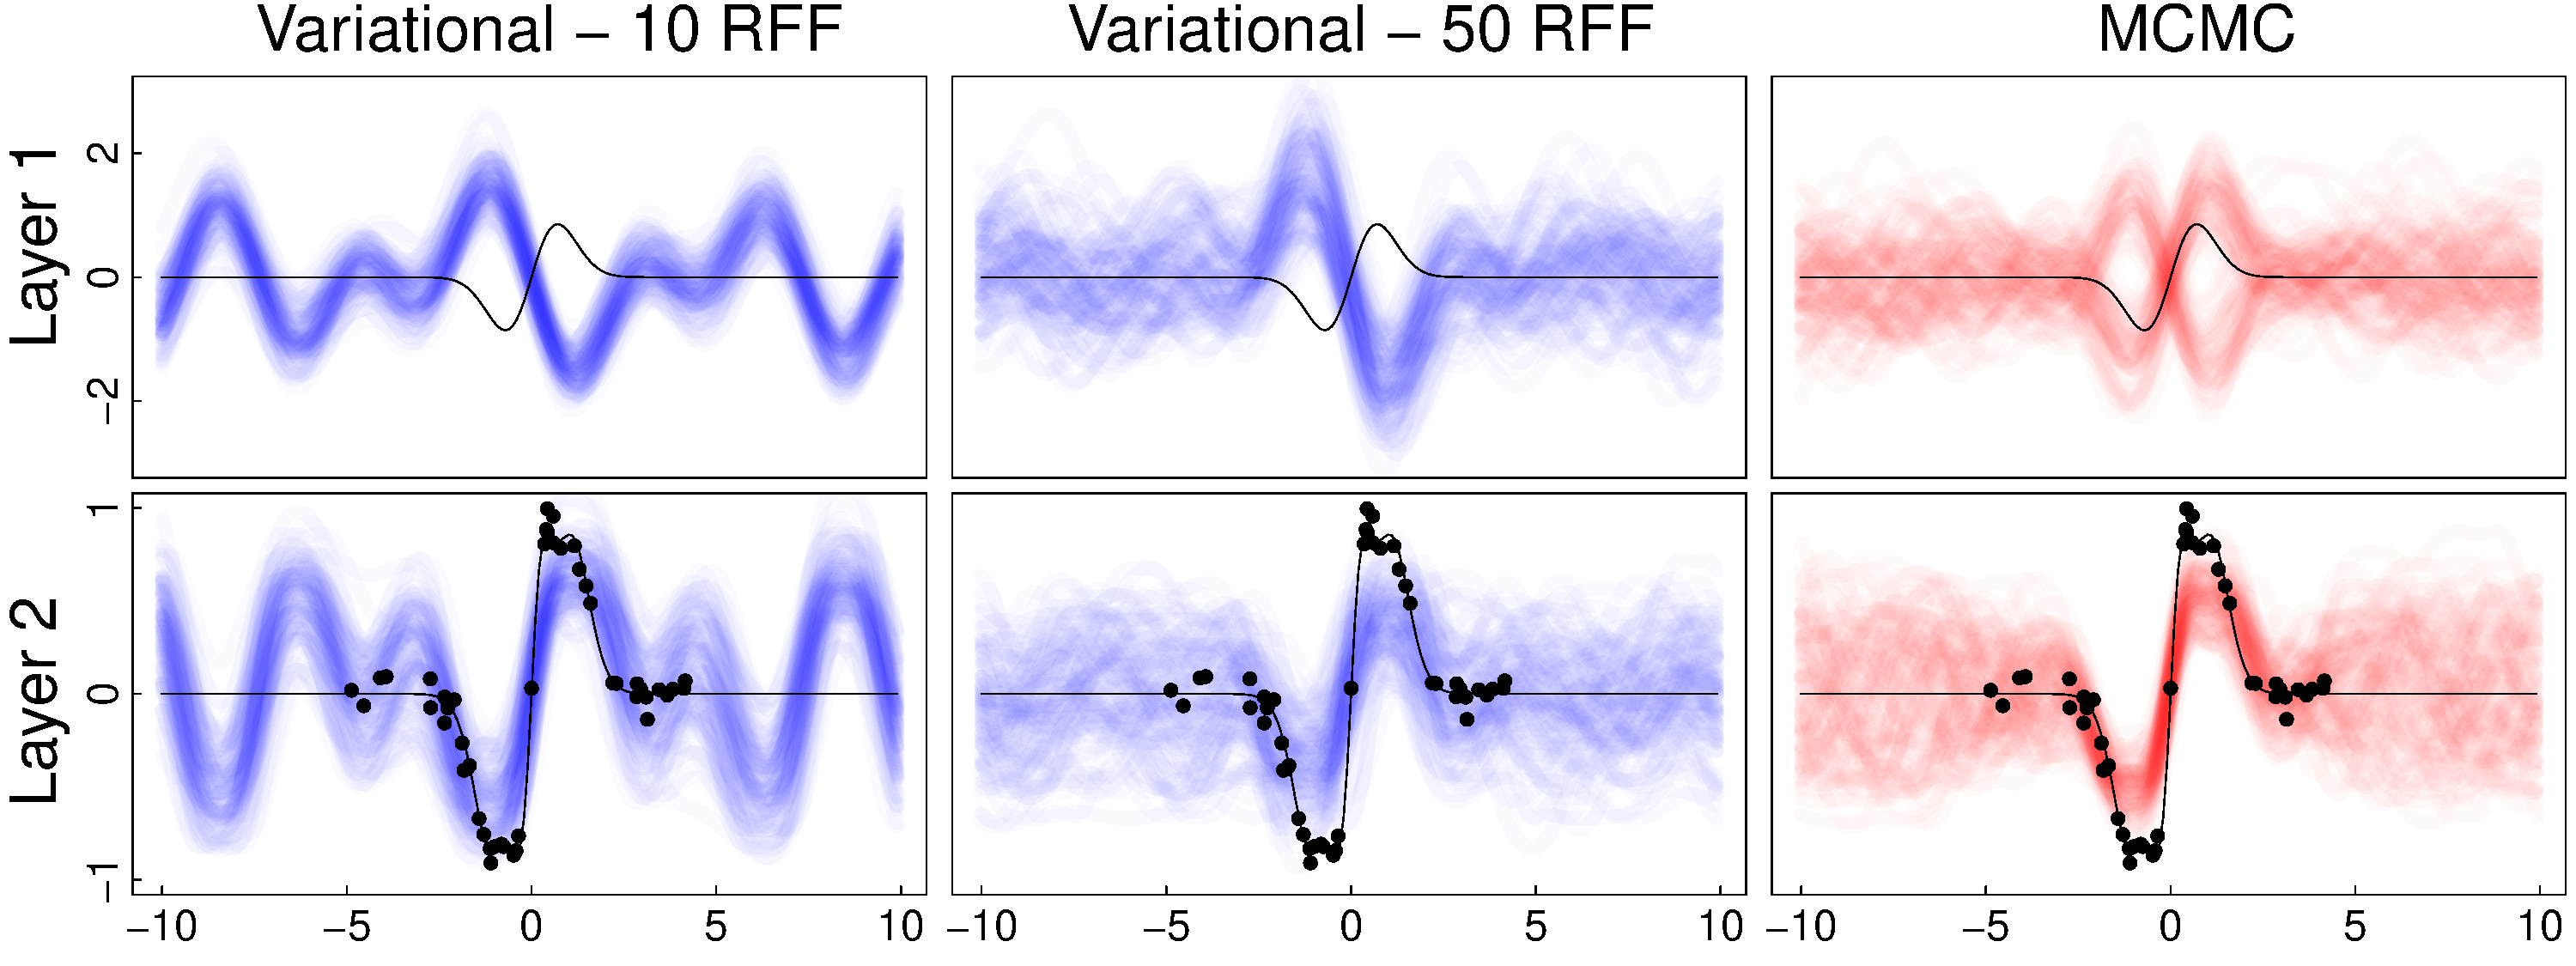
\includegraphics[width=10cm]{figures/figure_compare_MCMC_var.pdf}
}
%% \vspace{.3in}
\caption{
Comparison of \mcmc and variational inference of a two-layer \dgp with a single \gp in the hidden layer and a Gaussian likelihood.
The posterior over the latent functions is based on $100$ \mcmc samples and $100$ samples from the variational posterior. 
%% The variational approximation is applied to the proposed approximate \dgp model with $10$ (left column) and $50$ (center column) random Fourier features.
}
\label{fig:compare_MCMC_variational}
\end{figure}

We obtained samples from the posterior over the latent variables at each layer using \mcmc techniques.
In the case of a Gaussian likelihood, it is possible to integrate out the \gp at the last layer, thus obtaining a model that only depends on the \gp at the first.
As a result, the collapsed \dgp model becomes a standard \gp model whose latent variables can be sampled using various \mcmc samplers developed in the literature of \mcmc for \gp{s}.
Here we employ Elliptical Slice Sampling~\cite{Murray10b} to draw samples from the posterior over the latent variables at the first layer, whereas latent variables at the second can be sampled directly from a multivariate Gaussian distribution.
More details on the \mcmc sampler are reported at the end of this section.

The plots depicted in Figure~\ref{fig:compare_MCMC_variational} illustrate how the \mcmc approach explores two modes of the posterior of opposite sign. 
This is due to the output function being invariant to the flipping of the sign of the weights at the two layers.
Conversely, the variational approximation over $\Wvect$ accurately identifies one of the two modes of the posterior.
The overall approximation is accurate in the case of more random Fourier features, whereas in the case of less, the approximation is unsurprisingly characterized by out-of-sample oscillations.
The variational approximation seems to result in larger uncertainty in predictions compared to \mcmc; we attribute this to the factorization of the posterior over all the weights.



\subsection{Details of \mcmc sampler for a two-layer \dgp with a Gaussian likelihood}

We give details of the \mcmc sampler that we used to draw samples from the posterior over latent variables in \dgp{s}.
In the experiments, we regard this as the gold-standard against which we compare the quality of the proposed \dgp approximation and inference. 
For the sake of tractability, we assume a two-layer \dgp with a Gaussian likelihood, and we fix the hyper-parameters of the GPs.
Without loss of generality, we assume $Y$ to be univariate and the hidden layer to be composed of a single GP.
The model is therefore as follows:
\begin{eqnarray}
p\left(Y \middle| F^{(2)}, \lambda\right) & = & \norm\left( Y \middle| F^{(2)}, \lambda I \right) \nonumber \\
p\left(F^{(2)} \middle| F^{(1)}, \thetavect^{(1)}\right) & = & \norm\left( F^{(2)} \middle| \zerovect, K\left(F^{(1)}, \thetavect^{(1)}\right) \right)  \nonumber \\
p\left(F^{(1)} \middle| X, \thetavect^{(0)}\right) & = & \norm\left( F^{(1)} \middle| \zerovect, K\left(X, \thetavect^{(0)}\right) \right)  \nonumber 
\end{eqnarray}
with $\lambda$, $\thetavect^{(1)}$, and $\thetavect^{(0)}$ fixed.
In the model specification above, we denoted by $K\left(F^{(1)}, \thetavect^{(1)}\right)$ and $K\left(X, \thetavect^{(0)}\right)$ the covariance matrices obtained by applying the covariance function with parameters $\thetavect^{(1)}$, and $\thetavect^{(0)}$ to all pairs of $F^{(1)}$ and $X$, respectively.

%% Define
%% \begin{eqnarray}
%% K^{(1)} & = & K\left(F^{(1)}, \thetavect^{(1)}\right)  \nonumber \\
%% K^{(0)} & = & K\left(X, \thetavect^{(0)}\right)  \nonumber 
%% \end{eqnarray}
Given that the likelihood is Gaussian, it is possible to integrate out $F^{(2)}$ analytically
$$
p\left(Y \middle| F^{(1)}, \lambda, \thetavect^{(1)}\right) = \int p\left(Y \middle| F^{(2)}, \lambda\right) p\left(F^{(2)} \middle| F^{(1)}, \thetavect^{(1)}\right) dF^{(2)}
$$
obtaining the more compact model specification:
\begin{eqnarray}
p\left(Y \middle| F^{(1)}, \lambda, \thetavect^{(1)}\right) & = & \norm\left( Y \middle| \zerovect, K\left(F^{(1)}, \thetavect^{(1)}\right) + \lambda I \right) \nonumber \\
p\left(F^{(1)} \middle| X, \thetavect^{(0)}\right) & = & \norm\left( F^{(1)} \middle| \zerovect, K\left(X, \thetavect^{(0)}\right) \right)  \nonumber
\end{eqnarray}
For fixed hyper-parameters, these expressions reveal that the observations are distributed as in the standard GP regression case, with the only difference that the covariance is now parameterized by GP distributed random variables $F^{(1)}$. 
We can interpret these variables as some sort of hyper-parameters, and we can attempt to use standard \mcmc methods to samples from their posterior.

In order to develop a sampler for all latent variables, we factorize their full posterior as follows:
$$
p\left(F^{(2)}, F^{(1)} \middle| Y, X, \lambda, \thetavect^{(1)}, \thetavect^{(0)}\right) = 
p\left(F^{(2)} \middle| Y, F^{(1)}, \lambda, \thetavect^{(1)}\right) p\left(F^{(1)} \middle| Y, X, \lambda, \thetavect^{(1)}, \thetavect^{(0)}\right)
$$
which suggest a Gibbs sampling strategy to draw samples from the posterior where we iterate
\begin{enumerate}
	\item 
	sample from 
	$
	p\left(F^{(1)} \middle| Y, X, \lambda, \thetavect^{(1)}, \thetavect^{(0)}\right)
	$
	\item
	sample from 
	$
	p\left(F^{(2)} \middle| Y, F^{(1)}, \lambda, \thetavect^{(1)}\right)
	$
\end{enumerate}

Step 1. can be done by setting up a Markov chain with invariant distribution given by:
$$
p\left(F^{(1)} \middle| Y, X, \lambda, \thetavect^{(1)}, \thetavect^{(0)}\right) \propto p\left(Y \middle| F^{(1)}, \lambda, \thetavect^{(1)}\right) p\left(F^{(1)} \middle| X, \thetavect^{(0)}\right)
$$
We can interpret this as a GP model, where the likelihood now assumes a complex form because of the nonlinear way in which the likelihood depends on $F^{(1)}$.
Because of this interpretation, we can attempt to use any of the samplers developed in the literature of GPs to obtain samples from the posterior over latent variables in GP models.

Step 2. can be done directly given that the posterior over $F^{(2)}$ is available in closed form and it is Gaussian:
$$
p\left(F^{(2)} \middle| Y, F^{(1)}, \lambda, \thetavect^{(1)}\right) = \norm
\left(F^{(2)} \middle| 
K^{(1)} \left(K^{(1)} + \lambda I\right)^{-1} Y,
K^{(1)} - K^{(1)} \left(K^{(1)} + \lambda I\right)^{-1} K^{(1)}
\right)
$$
where we have defined
$$
K^{(1)} := K\left(F^{(1)}, \thetavect^{(1)}\right)
$$





\section{Derivation of the lower bound}

For the sake of completeness, here is a detailed derivation of the lower bound that we use in variational inference to learn the posterior over $\Wvect$ and optimize $\Thetavect$, assuming $\Omegavect$ fixed:
\begin{eqnarray}
\log [p(Y | X, \Omegavect, \Thetavect)] & = & \log\left[ \int p(Y | X, \Wvect, \Omegavect, \Thetavect) p(\Wvect) d \Wvect \right] \nonumber \\
& = & \log\left[ \int \frac{p(Y | X, \Wvect, \Omegavect, \Thetavect) p(\Wvect)}{q(\Wvect)} q(\Wvect) d\Wvect \right] \nonumber \\
& = & \log\left[ \E_{q(\Wvect)} \frac{p(Y | X, \Wvect, \Omegavect, \Thetavect) p(\Wvect)}{q(\Wvect)} \right] \nonumber \\
& \geq & \E_{q(\Wvect)} \left( \log\left[ \frac{p(Y | X, \Wvect, \Omegavect, \Thetavect) p(\Wvect)}{q(\Wvect)} \right] \right) \nonumber \\
& = & \E_{q(\Wvect)} \left( \log[ p(Y | X, \Wvect, \Omegavect, \Thetavect) ] \right) + \E_{q(\Wvect)} \left( \log\left[\frac{ p(\Wvect)}{q(\Wvect)} \right] \right) \nonumber \\
& = & \E_{q(\Wvect)} \left( \log[ p(Y | X, \Wvect, \Omegavect, \Thetavect) ] \right) - \mathrm{DKL}[q(\Wvect) || p(\Wvect)] \nonumber
\end{eqnarray}

\section{Learning $\Omegavect$ variationally}

Defining $\Psivect = \{\Wvect, \Omegavect\}$, we can attempt to employ variational inference to treat the spectral frequencies $\mathbf{\Omegavect}$ variationally as well as $\Wvect$. 
In this case, the detailed derivation of the lower bound is as follows:
\begin{eqnarray}
\log \left[p(Y \middle| X, \Thetavect)\right] & = & \log\left[ \int p(Y | X, \Psivect, \Thetavect) p(\Psivect | \Thetavect) d\Psivect \right] \nonumber \\
& = & \log\left[ \int \frac{p(Y | X, \Psivect, \Thetavect) p(\Psivect | \Thetavect)}{q(\Psivect)} q(\Psivect) d\Psivect \right] \nonumber \\
& = & \log\left[ \E_{q(\Psivect)} \frac{p(Y | X, \Psivect, \Thetavect) p(\Psivect | \Thetavect)}{q(\Psivect)} \right] \nonumber \\
& \geq & \E_{q(\Psivect)} \left( \log\left[ \frac{p(Y | X, \Psivect, \Thetavect) p(\Psivect | \Thetavect)}{q(\Psivect)} \right] \right) \nonumber \\
& = & \E_{q(\Psivect)} \left( \log[ p(Y | X, \Psivect, \Thetavect) ] \right) + \E_{q(\Psivect)} \left( \log\left[\frac{ p(\Psivect | \Thetavect)}{q(\Psivect)} \right] \right) \nonumber \\
& = & \E_{q(\Psivect)} \left( \log[ p(Y | X, \Psivect, \Thetavect) ] \right) - \mathrm{DKL}[q(\Psivect) || p(\Psivect | \Thetavect)] \nonumber
\end{eqnarray}

Again, assuming a factorized prior over all weights across layers
\begin{equation}
p(\Psivect | \thetavect) = \prod_{l=0}^{N_{\mathrm{h}} - 1} p(\Omega^{(l)} | \thetavect^{(l)}) p(W^{(l)}) = \prod_{ijl} q\left(\Omega^{(l)}_{ij}\right) \prod_{ijl} q\left(W^{(l)}_{ij}\right) \text{,}
\end{equation}
we optimize the variational lower bound using variational inference following the mini-batch approach with the reparameterization trick explained in the main paper.
%% The variational lower bound is as follows:
%% \begin{equation}
%% \LL \geq \E_{q(\Psivect)} \left( \log\left[ p\left(Y | \Psivect\right) \right] \right) - \mathrm{DKL}\left[q(\Psivect) \| p\left(\Psivect | \thetavect\right)\right] \text{,}
%% \end{equation}
%% where $q(\Psivect)$ acts as an approximation to the posterior over all the weights $p(\Psivect | Y, X, \thetavect)$.
%% %% In the equations above, we introduced a distribution over the parameters $q(\Psi)$ that acts as an approximation to the posterior over all the weights $p(\Psi | Y, \thetavect)$. % and spectral frequencies $\Psi = (\Psi^{(0)}, \ldots, \Psi^{(N_{\Psi})})$.
%% %% We used Jensen's inequality to bound the marginal likelihood, obtaining a standard lower bound as the difference between the expected value of the likelihood under the approximating distribution, and the Kullback-Leibler divergence between the prior and the approximating distribution.
%% We assume that the approximating distribution factorizes across layers, spectral frequencies and weights:
%% \begin{equation}
%% q(\Psivect) 
%% \end{equation}
%% %% \begin{eqnarray}
%% %% q(\Psi) & = & \prod_{ij} q\left(\Omega^{(0)}_{ij}\right) \cdots \prod_{ij} q\left(\Omega^{(N_{\mathrm{h}} - 1)}_{ij}\right) \times \nonumber \\
%% %% && \prod_{ij} q\left(W^{(0)}_{ij}\right) \cdots \prod_{ij} q\left(W^{(N_{\mathrm{h}} - 1)}_{ij}\right) \nonumber \text{.}
%% %% \end{eqnarray}
The variational parameters then become the mean and the variance of each of the approximating factors
\begin{equation}
q\left(W^{(l)}_{ij}\right) = \norm\left(m^{(l)}_{ij}, (s^2)^{(l)}_{ij} \right) \text{,}
%% q\left(W^{(l)}_{ij}\right) = \norm\left(W^{(l)}_{ij} \left\rvert \mu^{(l)}_{ij}, (\sigma^2)^{(l)}_{ij} \right. \right)
\end{equation}
\begin{equation}
q\left(\Omega^{(l)}_{ij}\right) = \norm\left(\mu^{(l)}_{ij}, (\beta^2)^{(l)}_{ij} \right) \text{,}
%% q\left(W^{(l)}_{ij}\right) = \norm\left(W^{(l)}_{ij} \left\rvert \mu^{(l)}_{ij}, (\sigma^2)^{(l)}_{ij} \right. \right)
\end{equation}
and we optimize the lower bound with respect to the variational parameters $m^{(l)}_{ij}, (s^2)^{(l)}_{ij}, \mu^{(l)}_{ij}, (\beta^2)^{(l)}_{ij}$. % for all $i, j, l$.



\section{Expression for the DKL divergence between Gaussians}

Given $p_1(x) = \norm(\mu_1, \sigma^2_1)$ and $p_2(x) = \norm(\mu_2, \sigma^2_2)$, the KL divergence between the two is:
%% Given $p_1(x) = \norm(x | \mu_1, \sigma^2_1)$ and $p_2(x) = \norm(x | \mu_2, \sigma^2_2)$, the KL divergence between the two is:
$$
\mathrm{DKL}\left(p_1(x) \| p_2(x)\right) = \frac{1}{2} 
\left[
\log\left(\frac{\sigma^2_2}{\sigma^2_1}\right) 
-1 
+ \frac{\sigma^2_1}{\sigma^2_2}
+ \frac{(\mu_1 - \mu_2)^2}{\sigma^2_2}
\right]
$$ 


\section{Distributed Implementation}

Our model is easily amenable to a distributed implementation using asynchronous distributed stochastic gradient descent~\citet{Chilimbi14}. % \citep{Chilimbi14, MartinAbadi15}. 
Our distributed setting, % \footnote{Currently, we use a CPU-only compute cluster.}
based on TensorFlow, includes one or more \emph{Parameter servers} (\name{ps}), and a number of \emph{Workers}. 
The latter proceed asynchronously using randomly selected batches of data: they fetch fresh model parameters from the \name{ps}, compute the gradients of the lower bound with respect to these parameters, and push those gradients back to the \name{ps}, which update the model accordingly. 
Given that workers compute gradients and send updates to \name{ps} asynchronously, the  discrepancy between the model used to compute gradients and the model actually updated can degrade training quality. 
This is exacerbated by a large number of asynchronous workers, as noted in~\citet{Chen16}.

We focus our experiments on the MNIST dataset, and study how training time and error rates evolve with the number of workers introduced in our system. 
The parameters for the model are identical to those reported for the previous experiments.

\pgfplotsset{label style={font=\Large}, title style={font=\Large}}
%\pgfplotsset{label style={font=\Large}, title style={font=\Large}}

\begin{figure}[ht]
\begin{center}
%% \begin{tabular}{c}
 {\scriptsize \bf  MNIST} \\
%% {\small MNIST-8M}\\
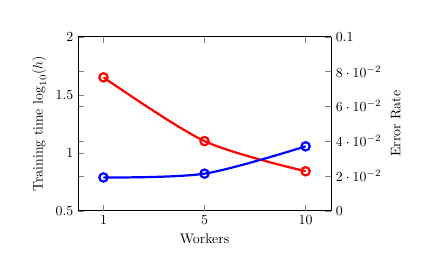
\begin{tikzpicture}[scale=0.5]
\begin{axis}[
    xmin=0, xmax=4,
  axis y line*=left,
	width=8cm, height=6cm,
  ylabel={Training time $\log_{10}(h)$},
  ymin=0.5, ymax=2,
  xlabel=Workers,
  xmin = 0.75, xmax = 3.25,
  xtick= {1,2,3},
  xticklabels={},
  extra x ticks={1,2,3},
  extra x tick style={xticklabels={1,5,10}}
  %xticklabels={0,1,5,10,15},
]
\addplot[smooth, mark=o, mark size=3pt, red, ultra thick]
coordinates{
    (1,1.65)
    (2,1.10)
    (3,0.84)
}; \label{plot_one}
%\addlegendentry{plot 1}
\end{axis}

\begin{axis}[
	width=8cm, height=6cm,
  ylabel={Error Rate},
  axis x line=none,
  xmin = 0.75, xmax = 3.25,
  ymin=0, ymax=0.1,
  ylabel near ticks, yticklabel pos=right
%% axis y line*=right
]
\addplot[smooth, mark=o, mark size=3pt, blue, ultra thick]
  coordinates{
    (1,0.0191)
    (2,0.0213)
    (3,0.037)
}; \label{plot_two}
%\addlegendimage{/pgfplots/refstyle=plot_one}\addlegendentry{plot 1}
%\addlegendimage{/pgfplots/refstyle=plot_two}\addlegendentry{plot 2}
\end{axis} 
\end{tikzpicture} 
%% &
%% \begin{tikzpicture}[scale=0.32]
%% \pgfplotsset{
%%     scale only axis,
%%     xmin=0, xmax=4
%% }

%% \begin{axis}[
%%   axis y line*=left,
%%   ylabel={Training time},
%%   ymin=6, ymax=17,
%%   xlabel=Workers,
%%   xmin = 0.75, xmax = 3.25,
%%   xtick= {1,2,3},
%%   xticklabels={},
%%   extra x ticks={1,2,3},
%%   extra x tick style={xticklabels={1,5,10}}
%%   %xticklabels={0,1,5,10,15},
%% ]
%% \addplot[smooth, mark=o, mark size=3pt, red, ultra thick]
%%   coordinates{
%%     (1,16)
%%     (2,12.6)
%%     (3,8)
%% }; \label{plot_one}
%% %\addlegendentry{plot 1}
%% \end{axis}

%% \begin{axis}[
%%   axis y line*=right,
%%   ylabel={Error Rate},
%%   axis x line=none,
%%   xmin = 0.75, xmax = 3.25,
%%   ymin=0, ymax=0.22
%% ]
%% \addplot[smooth, mark=o, mark size=3pt, blue, ultra thick]
%%   coordinates{
%%     (1,0.01)
%%     (2,0.04)
%%     (3,0.15)
%% }; \label{plot_two}
%% %\addlegendimage{/pgfplots/refstyle=plot_one}\addlegendentry{plot 1}
%% %\addlegendimage{/pgfplots/refstyle=plot_two}\addlegendentry{plot 2}
%% \end{axis} 
%% \end{tikzpicture}\\
%% \multicolumn{1}{c}{
\includegraphics[width=150pt]{figures/legend_async.pdf}
%% }
%% \end{tabular}
\end{center}
\caption{Comparison of training time and error rate for asynchronous \name{dgp-rbf} with 1, 5 and 10 workers.}
\label{fig:async}
\end{figure}


We report the results in Figure~\ref{fig:async}, and as expected, the training time decreases in proportion to the number of workers, albeit sub-linearly.
On the other hand, the increasing error rate confirms our intuition that imprecise updates of the gradients negatively impact the optimization procedure. 
The work in~\citet{Chen16} corroborates our findings, and motivates efforts in the direction of alleviating this issue.


\end{document}